\RequirePackage{fix-cm}
\documentclass[10pt,aspectratio=169]{beamer}
\usetheme[progressbar=none,block=fill]{metropolis}
\geometry{paperwidth=180mm,paperheight=101.25mm}
\usepackage{booktabs,tabularx,array,listings,tikz}
\definecolor{ink}{HTML}{17343B}
\definecolor{accent}{HTML}{007F78}
\definecolor{muted}{HTML}{52666C}
\definecolor{mist}{HTML}{F0F4F4}
\setbeamercolor{normal text}{fg=ink,bg=white}
\setbeamercolor{alerted text}{fg=accent}
\setbeamercolor{frametitle}{fg=white,bg=ink}
\setbeamercolor{progress bar}{fg=accent,bg=mist}
\setbeamercolor{block title}{fg=accent,bg=mist}
\setbeamercolor{block body}{fg=ink,bg=mist}
\setbeamertemplate{navigation symbols}{}
\setbeamertemplate{frame footer}{Mathis Clément\enspace |\enspace HSG · HS2026\enspace |\enspace English draft}
\setbeamertemplate{frame numbering}{\insertframenumber/19}
\setbeamerfont{frametitle}{size=\large}
\pdfstringdefDisableCommands{\def\enspace{ }\def\translate#1{#1}}
\setbeamersize{text margin left=8mm,text margin right=8mm}
\setbeameroption{hide notes}
\newcommand{\sources}[1]{\par\vfill{\fontsize{6.5}{7.8}\selectfont\color{muted}#1\par}}
\newcommand{\keyline}[1]{\par\medskip{\large\color{accent}\bfseries #1}\par}
\newcommand{\code}[1]{\texttt{\detokenize{#1}}}
\newcommand{\confirm}[1]{{\small\textbf{AUTHOR CONFIRMATION REQUIRED:} #1}}
\newcommand{\erdetail}{0}
\renewcommand{\arraystretch}{1.18}
\renewcommand{\tabularxcolumn}[1]{>{\raggedright\arraybackslash}p{#1}}
\lstset{language=SQL,basicstyle=\linespread{1}\ttfamily\fontsize{8}{9.4}\selectfont,
  keywordstyle=\color{accent}\bfseries,commentstyle=\color{muted},
  stringstyle=\color{ink},showstringspaces=false,breaklines=true,
  columns=fullflexible,keepspaces=true,aboveskip=3pt,belowskip=3pt,
  frame=none,tabsize=2}
% Editable native TikZ diagrams. All dimensions are in centimetres.
\usetikzlibrary{arrows.meta,positioning,calc,shapes.geometric,fit}
% Six-sided event with rectangular text area and cardinal anchors.
\makeatletter
\pgfdeclareshape{epcevent}{
  \inheritsavedanchors[from=rectangle]
  \inheritanchorborder[from=rectangle]
  \inheritanchor[from=rectangle]{center}
  \inheritanchor[from=rectangle]{text}
  \inheritanchor[from=rectangle]{north}
  \inheritanchor[from=rectangle]{south}
  \inheritanchor[from=rectangle]{east}
  \inheritanchor[from=rectangle]{west}
  \backgroundpath{
    \northeast \pgf@xa=\pgf@x \pgf@ya=\pgf@y
    \southwest \pgf@xb=\pgf@x \pgf@yb=\pgf@y
    \pgfpathmoveto{\pgfpoint{\pgf@xb}{0pt}}
    \pgfpathlineto{\pgfpoint{\pgf@xb+5pt}{\pgf@ya}}
    \pgfpathlineto{\pgfpoint{\pgf@xa-5pt}{\pgf@ya}}
    \pgfpathlineto{\pgfpoint{\pgf@xa}{0pt}}
    \pgfpathlineto{\pgfpoint{\pgf@xa-5pt}{\pgf@yb}}
    \pgfpathlineto{\pgfpoint{\pgf@xb+5pt}{\pgf@yb}}
    \pgfpathclose
  }
}
\makeatother
\tikzset{
  flow/.style={-{Stealth[length=1.7mm]},draw=ink,line width=.65pt},
  event/.style={shape=epcevent,draw=muted,fill=mist,minimum height=.65cm,text width=2.0cm,align=center,font=\linespread{1}\fontsize{8.5}{10}\selectfont,inner xsep=6pt,inner ysep=3pt},
  function/.style={rectangle,rounded corners=2pt,draw=accent,fill=accent!9,minimum height=.77cm,text width=2.0cm,align=center,font=\linespread{1}\fontsize{8.5}{10}\selectfont,inner sep=4pt},
  xor/.style={circle,draw=ink,fill=white,minimum size=.48cm,inner sep=0pt,font=\fontsize{7}{8}\selectfont\bfseries},
  role/.style={font=\linespread{1}\fontsize{7}{8}\selectfont,text=muted,align=center},
  entity/.style={rectangle,rounded corners=4pt,draw=accent,fill=accent!5,text width=3.35cm,align=left,font=\linespread{1}\fontsize{8.5}{10}\selectfont,inner sep=6pt},
  relation/.style={draw=ink,line width=.6pt},
  relabel/.style={font=\linespread{1}\fontsize{7.3}{8.5}\selectfont,fill=white,inner sep=1.5pt,text=ink,align=center},
  component/.style={rectangle,rounded corners=3pt,draw=accent,fill=accent!7,text width=3cm,minimum height=.9cm,align=center,font=\linespread{1}\small,inner sep=5pt}
}
\newcommand{\epclegend}{\par\smallskip{\fontsize{7}{8}\selectfont\color{muted}EPC: hexagon = state/event; rounded box = activity/function; arrow = control flow; XOR = exactly one branch. [Role] is an annotation.\par}}
\newcommand{\erlegend}{\par\smallskip{\fontsize{7}{8}\selectfont\color{muted}\# = identifier; * = mandatory attribute; o = optional (none here). Rounded entities follow VL03. Extension: explicit endpoint ranges replace line-style optionality/crow's feet; lines are non-directional relationships.\par}}

\title{Designing a Mileage-Based\\Electric Vehicle Tax System}
\subtitle{Case A: Electromobility\enspace |\enspace English review draft}
\author{Mathis Clément}
\institute{University of St. Gallen (HSG)\\Information and Communication Technology · HS2026}
\date{9 November 2026}
\hypersetup{pdftitle={Designing a Mileage-Based Electric Vehicle Tax System},pdfauthor={Mathis Clément},pdfsubject={HSG IKT HS2026 — English review draft}}

\begin{document}

% 1 — 15 seconds
\begin{frame}[plain]
\vspace{7mm}
{\LARGE\bfseries Designing a Mileage-Based\\Electric Vehicle Tax System\par}
\vspace{3mm}{\color{accent}\rule{\textwidth}{1pt}}\par
{\large Case A: Electromobility\par}
\medskip
\textbf{Mathis Clément}\par
University of St. Gallen (HSG)\\
Information and Communication Technology · HS2026
\par\medskip
{\small English review draft · 9 November 2026}
\end{frame}

% 2 — 40 seconds
\begin{frame}{Tax distance travelled, without tracking journeys}
\begin{columns}[T,onlytextwidth]
\column{.46\textwidth}
\begin{block}{The assignment's rates}
\textbf{BEV}: battery electric vehicle\\
\alert{3 pence per mile}\par\medskip
\textbf{PHEV}: plug-in hybrid electric vehicle\\
\alert{1.5 pence per mile}
\end{block}
\column{.51\textwidth}
\textbf{Four actors, distinct responsibilities}
\begin{itemize}\itemsep3pt
\item Owners declare mileage and pay.
\item MOT inspection centres verify readings.
\item DVLA supplies vehicle-registration data.
\item Tax authority assesses, settles and reports.
\end{itemize}
\end{columns}
\keyline{Estimate → advance → verified miles → settlement → management information}
{\small MOT = Ministry of Transport test. DVLA = Driver and Vehicle Licensing Agency; external reference authority in the design.}
\sources{[C] Cases IKT, HS2026, PDF p. 3. Rates and scenario are assignment inputs, not a claim about enacted UK law. No live agency connection is implemented.}
\end{frame}

% 3 — 50 seconds
\begin{frame}{A narrow scope makes the annual logic explainable}
\begin{tabularx}{\textwidth}{@{}p{.44\textwidth}X@{}}
\toprule
\textbf{Assumption} & \textbf{Design consequence}\\\midrule
One billing year: 1 Apr 2028–31 Mar 2029 & \code{period_end = 2029-04-01} is exclusive.\\
One unchanged owner; fixed rates; miles & No ownership or rate-period splits.\\
Verified readings at both boundaries; no reset & Closing minus opening gives actual miles.\\
One declaration and final assessment per vehicle/year & Assessment may be absent while work is in progress.\\
Integer pence; half-pennies upwards & Round once after mileage × rate.\\\bottomrule
\end{tabularx}\par
\medskip
\textbf{Boundary:} conceptual processes + local SQLite prototype, using fictional records.
\par\smallskip
{\small Excluded: website, authentication, real payments, live agencies, transfers, new-vehicle MOT exceptions, fraud, appeals, penalties and production deployment.}
\sources{[S] Scope.md, §§4–6. [L1] Modelling, PDF p. 54: purposeful reduction of detail. Calculation rules: A1.}
\end{frame}

% 4 — 50 seconds
\begin{frame}{Process 1 | An estimate creates an advance, not final tax}
\noindent{\small Accepted-declaration path; validation rejection is shown in the complete model, A2–A3.\par}
\begin{center}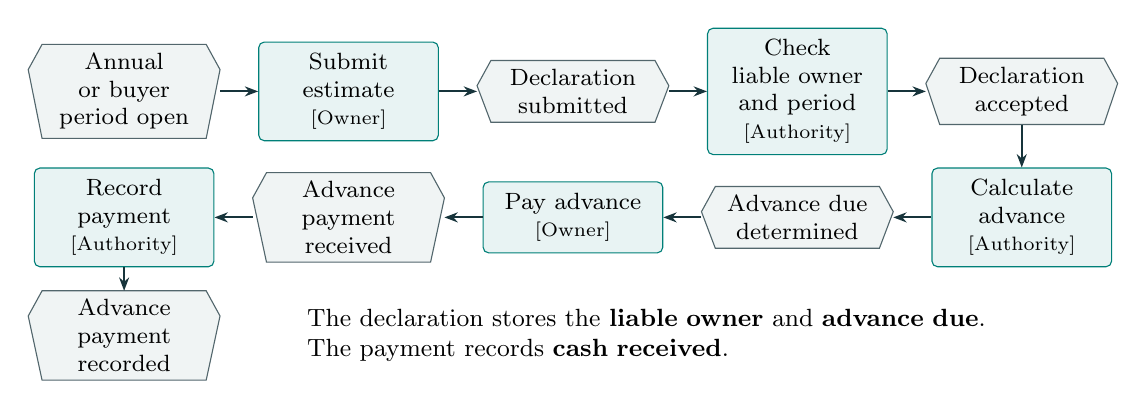
\begin{tikzpicture}
\node[event] (a) at (0,0) {Annual or buyer\\period open};
\node[function] (b) at (2.85,0) {Submit estimate\\{\scriptsize [Owner]}};
\node[event] (c) at (5.7,0) {Declaration\\submitted};
\node[function] (d) at (8.55,0) {Check liable owner\\and period\\{\scriptsize [Authority]}};
\node[event] (e) at (11.4,0) {Declaration\\accepted};
\node[function] (f) at (11.4,-1.6) {Calculate advance\\{\scriptsize [Authority]}};
\node[event] (g) at (8.55,-1.6) {Advance due\\determined};
\node[function] (h) at (5.7,-1.6) {Pay advance\\{\scriptsize [Owner]}};
\node[event] (i) at (2.85,-1.6) {Advance payment\\received};
\node[function] (j) at (0,-1.6) {Record payment\\{\scriptsize [Authority]}};
\node[event] (k) at (0,-3.1) {Advance payment\\recorded};
\foreach \s/\t in {a/b,b/c,c/d,d/e,e/f,f/g,g/h,h/i,i/j,j/k} \draw[flow] (\s)--(\t);
\node[align=left,text width=9cm,anchor=west,font=\small] at (2.2,-3.1) {The declaration stores the \textbf{liable owner} and \textbf{advance due}.\\The payment records \textbf{cash received}.};
\end{tikzpicture}
\end{center}
\epclegend
\sources{[L2] Processes, PDF pp. 21–25; [E] EPC cheat sheet, p. 1. Process design is supported by stored demonstration records, not an automated workflow.}
\end{frame}

% 5 — 60 seconds
\begin{frame}{Process 2 | Assessment and cash are separate events}
\begin{center}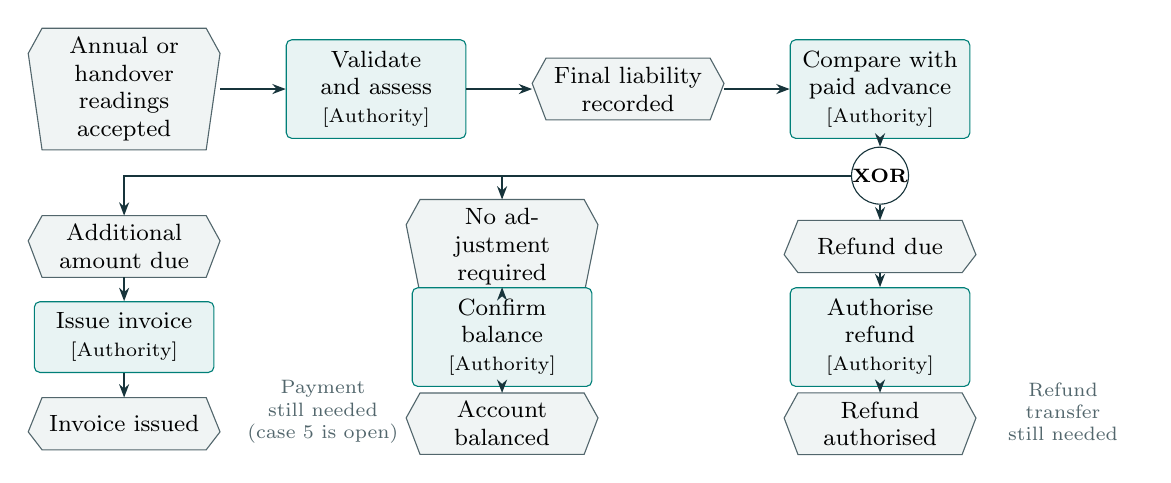
\begin{tikzpicture}
\node[event] (a) at (0,0) {Annual or handover\\readings accepted};
\node[function] (b) at (3.2,0) {Validate and assess\\{\scriptsize [Authority]}};
\node[event] (c) at (6.4,0) {Final liability\\recorded};
\node[function] (d) at (9.6,0) {Compare with\\paid advance\\{\scriptsize [Authority]}};
\node[xor] (x) at (9.6,-1.1) {XOR};
\foreach \s/\t in {a/b,b/c,c/d,d/x} \draw[flow] (\s)--(\t);
\node[event] (e) at (0,-2) {Additional\\amount due};
\node[event] (f) at (4.8,-2) {No adjustment\\required};
\node[event] (g) at (9.6,-2) {Refund due};
\draw[flow] (x.west)--(0,-1.1)--(e);
\draw[flow] (x.west)--(4.8,-1.1)--(f);
\draw[flow] (x)--(g);
\node[function] (h) at (0,-3.15) {Issue invoice\\{\scriptsize [Authority]}};
\node[function] (i) at (4.8,-3.15) {Confirm balance\\{\scriptsize [Authority]}};
\node[function] (j) at (9.6,-3.15) {Authorise refund\\{\scriptsize [Authority]}};
\node[event] (k) at (0,-4.25) {Invoice issued};
\node[event] (l) at (4.8,-4.25) {Account balanced};
\node[event] (m) at (9.6,-4.25) {Refund authorised};
\foreach \s/\t in {e/h,h/k,f/i,i/l,g/j,j/m} \draw[flow] (\s)--(\t);
\node[role,anchor=west,text width=2.1cm] at (1.35,-4.1) {Payment still needed\\(case 5 is open)};
\node[role,anchor=west,text width=1.8cm] at (10.9,-4.1) {Refund transfer\\still needed};
\end{tikzpicture}
\end{center}
\epclegend
\sources{Overview ends at authorisation. Full reading checks and cash-completion paths: A4–A5. [S] Scope.md; [L2] PDF pp. 21–25.}
\end{frame}

% 6 — 45 seconds
\begin{frame}{Process 3 | Validated aggregates support planning}
\noindent{\small Accepted-data path; quality rejection and the planning decision are detailed in A6–A7.\par}
\begin{center}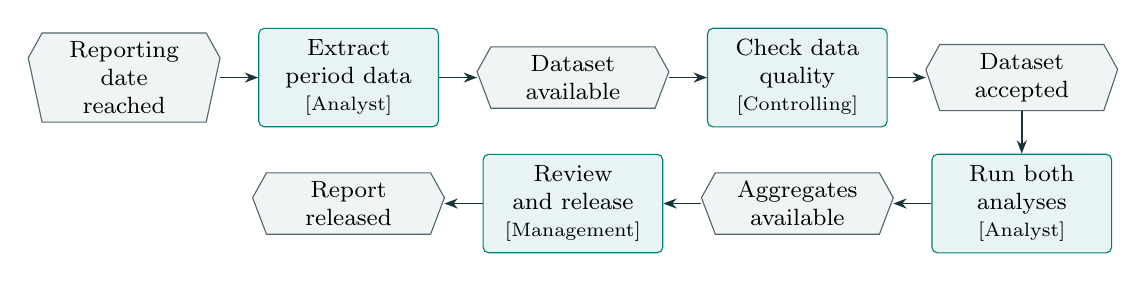
\begin{tikzpicture}
\node[event] (a) at (0,0) {Reporting date\\reached};
\node[function] (b) at (2.85,0) {Extract period data\\{\scriptsize [Analyst]}};
\node[event] (c) at (5.7,0) {Dataset\\available};
\node[function] (d) at (8.55,0) {Check data quality\\{\scriptsize [Controlling]}};
\node[event] (e) at (11.4,0) {Dataset\\accepted};
\node[function] (f) at (11.4,-1.6) {Run both analyses\\{\scriptsize [Analyst]}};
\node[event] (g) at (8.55,-1.6) {Aggregates\\available};
\node[function] (h) at (5.7,-1.6) {Review and release\\{\scriptsize [Management]}};
\node[event] (i) at (2.85,-1.6) {Report\\released};
\foreach \s/\t in {a/b,b/c,c/d,d/e,e/f,f/g,g/h,h/i} \draw[flow] (\s)--(\t);
\end{tikzpicture}
\end{center}
\begin{columns}[T,onlytextwidth]
\column{.48\textwidth}\textbf{Analysis 1: advance liability by type}\\Plan expected advances and understand mileage mix.
\column{.48\textwidth}\textbf{Analysis 2: gross settlement adjustments}\\Plan additional-assessment and refund workload.
\end{columns}
\epclegend
\sources{[L4] Databases and BI, PDF pp. 48–49. Implemented SQL: expected\_revenue.sql and additional\_tax.sql. Outstanding cash is a separate validation calculation.}
\end{frame}

% 7 — 70 seconds
\begin{frame}{Six entities connect responsibility, evidence and money}
\begin{center}% Six conceptual entities. FK attributes appear in the relational dictionary.
% Set \erdetail to 1 before input for the full attribute view.
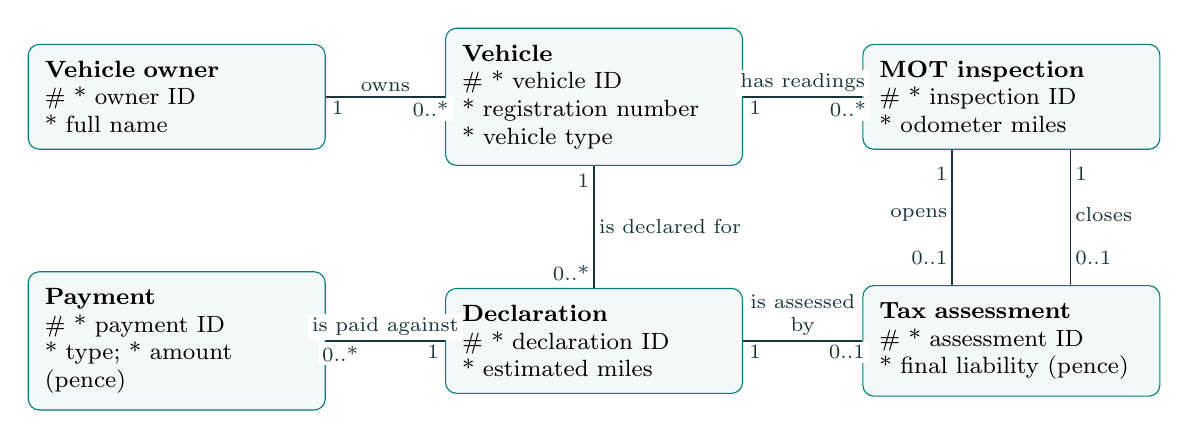
\begin{tikzpicture}
\node[entity] (o) at (0,0) {\textbf{Vehicle owner}\\\# * owner ID\\{}* full name\ifnum\erdetail=1\\{}* postal address\fi};
\node[entity] (v) at (5.3,0) {\textbf{Vehicle}\\\# * vehicle ID\\{}* registration number\\{}* vehicle type};
\node[entity] (i) at (10.6,0) {\textbf{MOT inspection}\\\# * inspection ID\\{}* odometer miles\ifnum\erdetail=1\\{}* inspection date\\{}* centre reference\fi};
\node[entity] (p) at (0,-3.1) {\textbf{Payment}\\\# * payment ID\\{}* type; * amount (pence)\ifnum\erdetail=1\\{}* paid timestamp\fi};
\node[entity] (d) at (5.3,-3.1) {\textbf{Declaration}\\\# * declaration ID\\{}* estimated miles\ifnum\erdetail=1\\{}* period start\\{}* period end (exclusive)\\{}* advance due (pence)\\{}* submitted at\fi};
\node[entity] (a) at (10.6,-3.1) {\textbf{Tax assessment}\\\# * assessment ID\\{}* final liability (pence)\ifnum\erdetail=1\\{}* assessed timestamp\fi};
\draw[relation] (o)--node[relabel,above]{owns} node[relabel,pos=.1,below]{1} node[relabel,pos=.88,below]{0..*}(v);
\draw[relation] (v)--node[relabel,above]{has readings} node[relabel,pos=.1,below]{1} node[relabel,pos=.88,below]{0..*}(i);
\draw[relation] (v)--node[relabel,right]{is declared for} node[relabel,pos=.12,left]{1} node[relabel,pos=.88,left]{0..*}(d);
\draw[relation] (p)--node[relabel,above]{is paid against} node[relabel,pos=.12,below]{0..*} node[relabel,pos=.9,below]{1}(d);
\draw[relation] (d)--node[relabel,above]{is assessed\\by} node[relabel,pos=.1,below]{1} node[relabel,pos=.87,below]{0..1}(a);
\draw[relation] ($(i.south)+(-.75,0)$)--node[relabel,pos=.18,left]{1} node[relabel,pos=.8,left]{0..1} node[relabel,pos=.48,left]{opens} ($(a.north)+(-.75,0)$);
\draw[relation] ($(i.south)+(.75,0)$)--node[relabel,pos=.18,right]{1} node[relabel,pos=.8,right]{0..1} node[relabel,pos=.48,right]{closes} ($(a.north)+(.75,0)$);
\end{tikzpicture}
\end{center}
\erlegend
\sources{[L3] Data modelling, PDF pp. 26–31, especially p. 28; [DB] schema and metadata. Ranges describe the entity at that endpoint, for one entity at the other end. Full attributes and inspection-role reuse: A8–A9.}
\end{frame}

% 8 — 40 seconds
\begin{frame}{SQLite implements the structure, not every business rule}
\begin{columns}[T,onlytextwidth]
\column{.47\textwidth}
\textbf{Six relations from six entities}
\begin{itemize}\itemsep3pt
\item \code{vehicle_owners}, \code{vehicles}
\item \code{declarations}, \code{mot_inspections}
\item \code{tax_assessments}, \code{payments}
\end{itemize}
\textbf{Implemented integrity}\\
Primary keys, foreign keys, mandatory fields and uniqueness constraints.
\column{.49\textwidth}
\textbf{Still a workflow responsibility}
\begin{itemize}\itemsep3pt
\item Same vehicle for declaration and readings.
\item Correct dates and non-decreasing mileage.
\item Allowed types and correct tax arithmetic.
\end{itemize}
\textbf{Storage choices}\\
Money: integer pence. Dates/timestamps: SQLite \code{TEXT}. Derived due/liability amounts are stored as an assessment record.
\end{columns}
\keyline{Inserted amounts are evidence of cases, not an automatic tax engine.}
\sources{[DB] scripts/setup\_database.py; PRAGMA metadata. Foreign-key enforcement must be enabled per connection. [L4] PDF pp. 15–18. Full mapping/schema: A10–A14.}
\end{frame}

% 9 — 65 seconds
\begin{frame}{Five cases exercise the same settlement process}
\begin{columns}[T,onlytextwidth]
\column{.60\textwidth}
\small
\begin{tabular}{@{}clrrl@{}}\toprule
Case & Type & Advance & Final & Outcome\\\midrule
1 & BEV & £300 & £360 & £60 extra, paid\\
2 & BEV & £300 & £240 & £60 refunded\\
3 & BEV & £300 & £300 & No adjustment\\
4 & PHEV & £120 & £150 & £30 extra, paid\\
5 & PHEV & £150 & £180 & \alert{£30 still owed}\\\bottomrule
\end{tabular}
\par\medskip
5 owners + 5 vehicles + 5 declarations +\\10 inspections + 5 assessments + 8 payments\\= \textbf{38 linked rows, five business cases}.
\column{.36\textwidth}
\begin{block}{Case 5: trace the balance}
22,000 − 10,000 = \textbf{12,000 miles}\par\smallskip
12,000 miles × 1.5 p/mile\\= 18,000 p = \textbf{£180}\par\smallskip
£180 liability − £150 received\\= \alert{£30 outstanding}
\end{block}
\end{columns}
\sources{[DB] Read-only recomputation of all five cases. All advances are paid; case 5 has no additional-payment record. Full evidence: A15–A17. Fictional examples, not a population estimate.}
\end{frame}

% 10 — 55 seconds
\begin{frame}[fragile]{Analysis 1 | Plan the advance liability by vehicle type}
\textbf{Question:} what advance amounts and mileage were declared for 2028/29?
\begin{center}
\begin{tabular}{@{}lcrrr@{}}\toprule
Start year & Type & Vehicles & Declared miles & Advance liability\\\midrule
2028 & BEV & 3 & 30,000 & £900.00\\
2028 & PHEV & 2 & 18,000 & £270.00\\\bottomrule
\end{tabular}
\end{center}
\begin{lstlisting}
FROM declarations AS d
JOIN vehicles AS v ON d.vehicle_id = v.vehicle_id
GROUP BY strftime('%Y', d.period_start), v.vehicle_type
\end{lstlisting}
\textbf{JOIN} supplies the type; \textbf{GROUP BY} forms year/type groups; sums give mileage and advance liability.
\keyline{£1,170 planned advances; a billing-year measure, not calendar-year cash.}
\sources{[Q1] database/queries/expected\_revenue.sql, executed unchanged. 2028/29 billing year, grouped by start year 2028. Original output alias: expected\_revenue\_gbp. Complete SQL/output: A18.}
\end{frame}

% 11 — 60 seconds
\begin{frame}[fragile]{Analysis 2 | Plan the scale of settlement adjustments}
\begin{center}
\begin{tabular}{@{}crrrrr@{}}\toprule
Start year & Assessed & Extra cases & Refund cases & Extra tax & Refunds\\\midrule
2028 & 5 & 3 & 1 & £120.00 & £60.00\\\bottomrule
\end{tabular}
\end{center}
\begin{lstlisting}
JOIN tax_assessments AS a ON d.declaration_id = a.declaration_id
SUM(CASE WHEN a.final_tax_pence > d.advance_due_pence
    THEN a.final_tax_pence - d.advance_due_pence ELSE 0 END)
\end{lstlisting}
{\small Excerpt: the conditional sum counts only positive differences; a second expression handles refunds.}
\medskip
\begin{columns}[T,onlytextwidth]
\column{.48\textwidth}\textbf{Planning meaning}\\Three additional assessments and one refund indicate settlement-processing work. One case needs no adjustment.
\column{.48\textwidth}\textbf{Cash distinction}\\The query does not join payments.\\\alert{£120 assessed ≠ £30 still outstanding.}
\end{columns}
\sources{[Q2] database/queries/additional\_tax.sql, executed unchanged. Comparison is with advance due (all paid in this sample). Full SQL/output: A19–A20; supplementary cash check: A21.}
\end{frame}

% 12 — 30 seconds
\begin{frame}{From a local prototype to a proposed operating architecture}
\begin{center}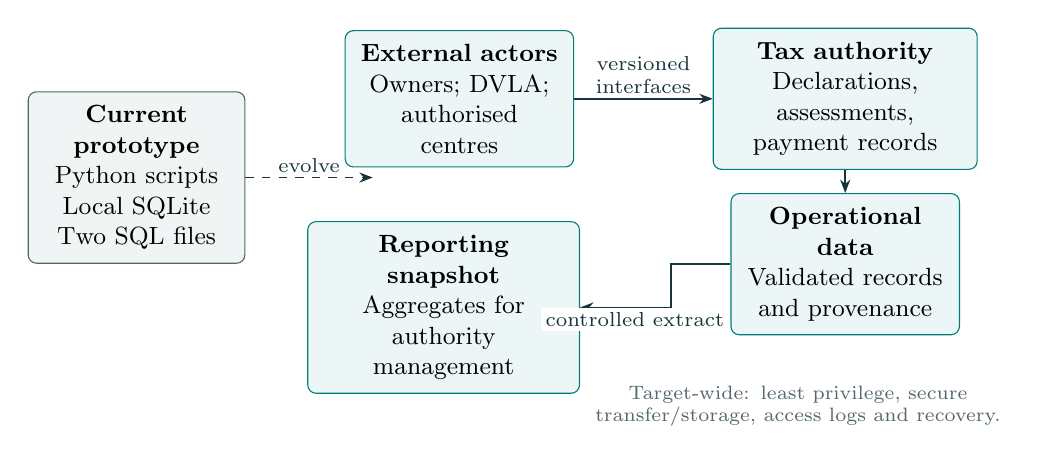
\begin{tikzpicture}
\node[component,text width=2.4cm,draw=muted,fill=mist] (now) at (0,0) {\textbf{Current prototype}\\Python scripts\\Local SQLite\\Two SQL files};
\node[component,text width=2.55cm] (actors) at (4.1,1) {\textbf{External actors}\\Owners; DVLA;\\authorised centres};
\node[component,text width=3cm] (ops) at (9,1) {\textbf{Tax authority}\\Declarations, assessments,\\payment records};
\node[component,text width=2.55cm] (data) at (9,-1.1) {\textbf{Operational data}\\Validated records\\and provenance};
\node[component,text width=3.1cm] (report) at (3.9,-1.65) {\textbf{Reporting snapshot}\\Aggregates for\\authority management};
\draw[flow] (actors)--node[relabel,above]{versioned\\interfaces}(ops);
\draw[flow] (ops)--(data);
\draw[flow] (data.west)--++(-.75,0)|-node[relabel,pos=.7,below]{controlled extract}(report.east);
\draw[flow,dashed] (now.east)--node[relabel,above]{evolve}(3,0);
\node[role,text width=5.4cm] at (8.4,-2.9) {Target-wide: least privilege, secure transfer/storage, access logs and recovery.};
\end{tikzpicture}
\end{center}
\textbf{Transition:} agree responsibilities and interfaces, validate operational processing, then introduce a reporting snapshot as load grows.
\sources{Target view: every component to the right of “Current prototype” is proposed. Arrows represent data exchange; dashed arrow represents evolution. [L5] PDF pp. 12, 15–16.}
\end{frame}

% 13 — 25 seconds
\begin{frame}{1 | Protect tax processing as workloads grow}
\begin{block}{Risk → principle}
Annual declaration peaks and heavy reports can slow or interrupt processing.\\
\textbf{Separate workloads and design critical processing for resilient growth.}
\end{block}
\textbf{Concrete decision:} run heavy management queries on a reporting snapshot; keep operational tax/payment processing recoverable.
\par\medskip
\textbf{Proposed validation:} test peak loads and recovery; if asynchronous transfers are added, retry the same payment without counting it twice.
\par\medskip
\textbf{Trade-off:} fresher reports cost more processing and operational effort. A snapshot introduces an explicit reporting delay.
\sources{Architecture chain 1 of 3. These are target decisions and tests, not achieved service levels. [L4] PDF pp. 48–49; [L5] pp. 12, 15–16; [L6] p. 18.}
\end{frame}

% 14 — 25 seconds
\begin{frame}{2 | Make responsibility for shared data explicit}
\begin{block}{Risk → principle}
Inconsistent identifiers, units and out-of-order records can create wrong assessments.\\
\textbf{Define authoritative ownership and standardised, versioned interfaces.}
\end{block}
\textbf{Concrete decision:} proposed ownership is DVLA for registration, MOT providers for verified readings, and the tax authority for assessments.
\par\medskip
\textbf{Proposed validation:} interface contracts require stable identifiers, miles, explicit dates and provenance; test duplicates and out-of-order readings before release.
\par\medskip
\textbf{Trade-off:} shared contracts reduce ambiguity but require partner coordination and version management.
\sources{Architecture chain 2 of 3. No live interfaces or automated cross-agency controls exist in the prototype. [L5] PDF pp. 12, 15–16; [L6] p. 18.}
\end{frame}

% 15 — 25 seconds
\begin{frame}{3 | Limit exposure of personal and financial data}
\begin{block}{Risk → principle}
More users, partners and reports increase opportunities for inappropriate access.\\
\textbf{Minimise personal data and enforce least-privilege access.}
\end{block}
\textbf{Concrete decision:} retain odometer totals, not journey/GPS histories; give management aggregates and operational roles only necessary records.
\par\medskip
\textbf{Proposed validation:} the authority assigns retention and access-review owners; test denied access and review logs. Protect data in transfer and storage.
\par\medskip
\textbf{Trade-off:} reduced access and retention limit ad-hoc investigation. Record which evidence is genuinely needed for an assessment.
\sources{Architecture chain 3 of 3. Access controls, encryption, logs and retention governance are proposed; legal compliance has not been established. [C] p. 3; [L5–L6].}
\end{frame}

% 16 — 45 seconds
\begin{frame}{AI reflection 1 | Assistance does not transfer responsibility}
\begin{columns}[T,onlytextwidth]
\column{.49\textwidth}
\textbf{Documented assistance}
\begin{itemize}\itemsep4pt
\item Explanations and drafts for scope, process/ER models, SQLite, sample data and SQL.
\item This English deck, diagram revisions, script, build and verification.
\end{itemize}
\textbf{Why useful:} quick alternatives and clear explanations for a small prototype.
\column{.47\textwidth}
\textbf{Human responsibility}
\begin{itemize}\itemsep4pt
\item Understand and defend the design and the meaning of each result.
\item Review the draft and acknowledge assistance.
\item Record the final narration personally; generated speech is prohibited.
\end{itemize}
\end{columns}
\medskip
\confirm{Which substantive activities did the author deliberately do without AI, and why? No historical non-use is inferred.}
\sources{[P] Supplied presentation brief: prior AI-use context. [C] PDF pp. 1–2, 4 (Task 7a). Separate HSG AI-use declaration is still required.}
\end{frame}

% 17 — 55 seconds
\begin{frame}{AI reflection 2 | A plausible label changed the business meaning}
\begin{columns}[T,onlytextwidth]
\column{.47\textwidth}
\begin{block}{AI-assisted original description}
“Outstanding amounts and refunds by period.”\par\smallskip
The reporting drawing proposes that output, but the implemented query compares \textbf{final tax with advance due}.
\end{block}
\column{.49\textwidth}
\begin{block}{Correction in this draft}
Label Analysis 2 \textbf{gross settlement adjustments}.\par\smallskip
Use signed payment totals for remaining balances:\\
£1,230 − (£1,170 + £90 − £60)\\
= \alert{£30 outstanding}.
\end{block}
\end{columns}
\textbf{Detection:} compare the proposed indicator with the query's tables and reconcile the payments. £120 is assessed extra tax; £90 has already been received.
\par\smallskip
\textbf{Course lesson:} integrated management information needs a precise business definition, not just valid SQL.
\sources{[D3] 03\_management\_reporting.drawio, queriesbody; file metadata agent=Codex supports AI-assisted provenance. [Q2], [DB]; [L4] PDF pp. 48–49. Comparison/correction performed by the presentation agent, not claimed as the author's independent discovery.}
\end{frame}

% 18 — 45 seconds
\begin{frame}{AI reflection 3 | Validate with the course, then claim only your work}
\textbf{Checks completed by the presentation agent}
\begin{itemize}\itemsep4pt
\item EPC: state/activity alternation, start/end events, XOR outcomes and role labels.
\item ER: endpoint cardinalities checked against keys, uniqueness and optional assessment.
\item SQLite: integrity and foreign-key checks passed; schema/data replay matched in memory.
\item Business meaning: all five mileage/rate calculations and signed payments reconciled.
\end{itemize}
\textbf{Why course knowledge matters:} foreign keys alone cannot validate the vehicle of both readings; a successful aggregate can still answer the wrong question.
\par\medskip
\confirm{Identify checks personally repeated and exclusively personal design decisions, with evidence. Simple code and English-first are documented preferences, not proof of independent system design.}
\sources{[L2–L4]; assets/database\_verification.json and editable diagram sources. Task 7c–7d: personal authorship statements remain specifically unresolved.}
\end{frame}

% 19 — 20 seconds
\begin{frame}{A traceable annual workflow, with a clear prototype boundary}
\keyline{Estimate → evidence → liability → cash → useful management information}
\begin{itemize}\itemsep9pt
\item Three process models connect to six SQLite tables and five settlement cases.
\item Two real SQL analyses support advance planning and settlement workload.
\item The key distinction holds: \textbf{£1,230 assessed = £1,200 net cash + £30 receivable}.
\end{itemize}
\medskip
\textbf{Limits:} one fictional year; exceptional cases and operational controls remain outside this prototype. Three architecture principles guide the next stage.
\sources{End of narrated English draft. Appendix A1–A23 contains complete models, implementation evidence, SQL, results and sources. Final course delivery requires German voice-over PowerPoint and separate database submission.}
\end{frame}

\appendix
\setcounter{framenumber}{0}
\setbeamertemplate{frame numbering}{A\insertframenumber}
% Unnarrated appendices A1–A23. Each frame is one PDF page.
\begin{frame}{A1 | Calculation rules and the billing boundary}
\small
\begin{tabularx}{\textwidth}{@{}p{.27\textwidth}X@{}}\toprule
Actual miles & Closing odometer miles − opening odometer miles.\\
Advance due (pence) & Estimated miles × rate (pence/mile), rounded once.\\
Final liability (pence) & Actual miles × rate (pence/mile), rounded once.\\
Net payments (pence) & Advances received + additional payments received − refunds paid.\\
Remaining balance (pence) & Final liability − net payments. Positive = owner owes; negative = refund owed.\\\bottomrule
\end{tabularx}\par
\medskip
\textbf{Period:} \code{[2028-04-01, 2029-04-01)}. The closing reading is taken at the exclusive upper boundary, covering distance through 31 March 2029.
\par\smallskip
\textbf{Rounding:} nearest penny, half upwards after multiplication. Example: 3 PHEV miles × 1.5 p/mile = 4.5 p → 5 p. Python's default \code{round()} does not guarantee this rule.
\par\smallskip
\textbf{Record semantics:} refunds store positive amounts and are subtracted. Due, assessed and paid are different measures. Current tax amounts were inserted, not automatically calculated.
\sources{[S] Scope.md, §§5–6; [DB] sample\_data.sql and read-only verification. BEV 3 p/mile; PHEV 1.5 p/mile, fixed throughout this demonstration.}
\end{frame}

\begin{frame}{A2 | Process 1, part 1: validate the declaration}
\begin{center}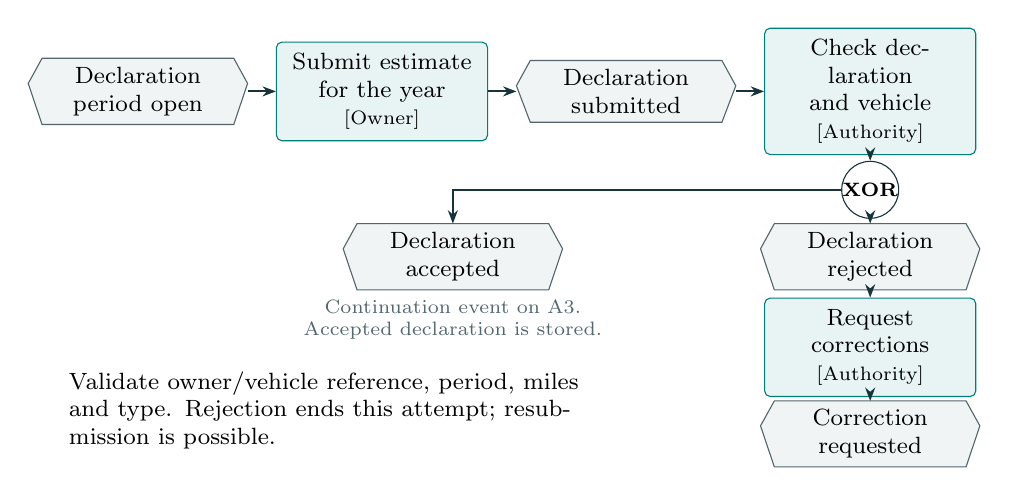
\begin{tikzpicture}[function/.append style={text width=2.4cm},event/.append style={text width=2.35cm}]
\node[event] (a) at (0,0) {Declaration\\period open};
\node[function] (b) at (3.1,0) {Submit estimate\\for the year\\{\scriptsize [Owner]}};
\node[event] (c) at (6.2,0) {Declaration\\submitted};
\node[function] (d) at (9.3,0) {Check declaration\\and vehicle\\{\scriptsize [Authority]}};
\node[xor] (x) at (9.3,-1.25) {XOR};
\node[event] (ok) at (4,-2.1) {Declaration\\accepted};
\node[event] (bad) at (9.3,-2.1) {Declaration\\rejected};
\node[function] (notify) at (9.3,-3.25) {Request\\corrections\\{\scriptsize [Authority]}};
\node[event] (end) at (9.3,-4.35) {Correction\\requested};
\foreach \s/\t in {a/b,b/c,c/d,d/x,x/bad,bad/notify,notify/end} \draw[flow] (\s)--(\t);
\draw[flow] (x.west)-|(ok.north);
\node[role,text width=4cm] at (4,-2.9) {Continuation event on A3.\\Accepted declaration is stored.};
\node[align=left,font=\fontsize{8.5}{10}\selectfont,text width=6.5cm,anchor=west] at (-1,-4.05) {Validate owner/vehicle reference, period, miles and type. Rejection ends this attempt; resubmission is possible.};
\end{tikzpicture}
\end{center}
\epclegend
\sources{Complete Process 1 spans A2–A3; repeated accepted event is a page continuation, not a second execution. [L2] PDF pp. 21–25; [E] p. 1.}
\end{frame}

\begin{frame}{A3 | Process 1, part 2: record actual advance cash}
\small
\begin{center}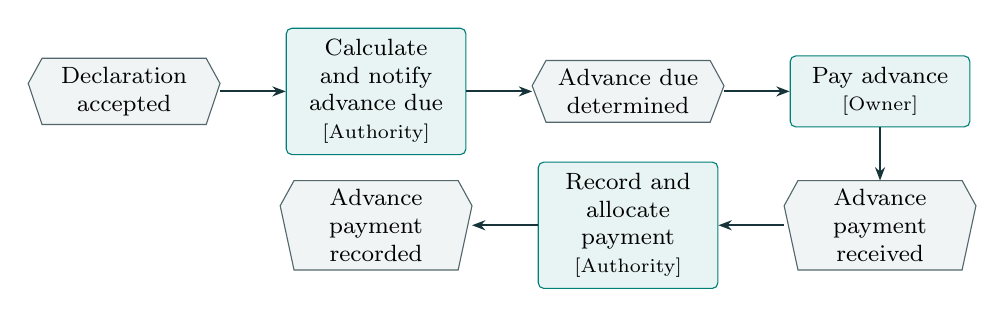
\begin{tikzpicture}
\node[event] (a) at (0,0) {Declaration\\accepted};
\node[function] (b) at (3.2,0) {Calculate and notify\\advance due\\{\scriptsize [Authority]}};
\node[event] (c) at (6.4,0) {Advance due\\determined};
\node[function] (d) at (9.6,0) {Pay advance\\{\scriptsize [Owner]}};
\node[event] (e) at (9.6,-1.7) {Advance payment\\received};
\node[function] (f) at (6.4,-1.7) {Record and allocate\\payment\\{\scriptsize [Authority]}};
\node[event] (g) at (3.2,-1.7) {Advance payment\\recorded};
\foreach \s/\t in {a/b,b/c,c/d,d/e,e/f,f/g} \draw[flow] (\s)--(\t);
\end{tikzpicture}
\end{center}
\begin{columns}[T,onlytextwidth]
\column{.48\textwidth}\textbf{Inputs and rules}\\Accepted estimate, vehicle type and period. Calculate miles × rate; round once half upwards.
\column{.48\textwidth}\textbf{Data effect}\\Store \code{advance_due_pence} in the declaration; create an \code{ADVANCE} payment when received.
\end{columns}
\medskip
{\small Payment failure and debt collection are outside the model. All five demonstration advances were received. Notification/payment activities are conceptual; only records are implemented.}
\epclegend
\sources{Continuation from A2. [S] Scope.md; [DB] sample\_data.sql; [L2], [E].}
\end{frame}

\begin{frame}{A4 | Process 2, part 1: evidence determines liability}
\begin{center}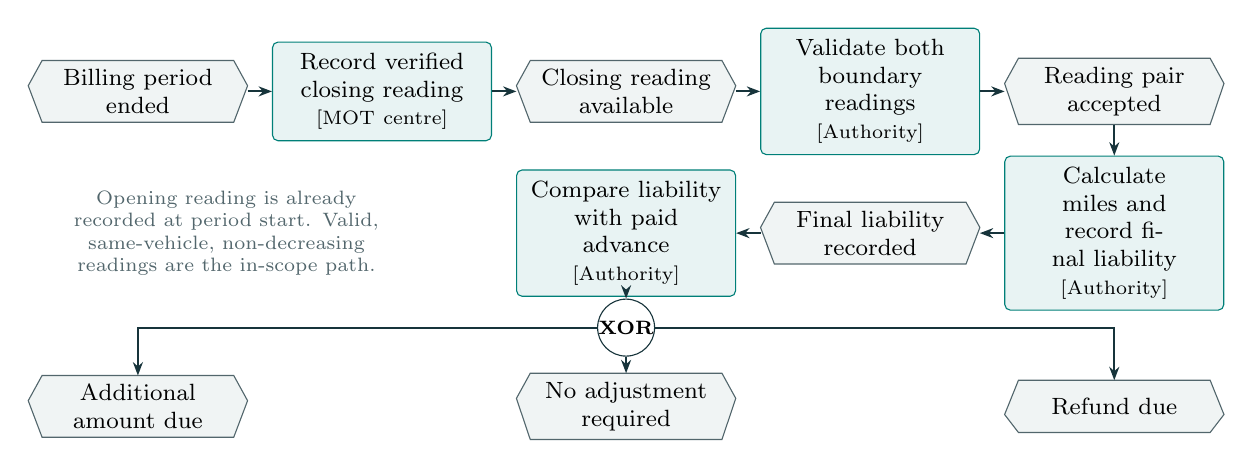
\begin{tikzpicture}[function/.append style={text width=2.5cm},event/.append style={text width=2.35cm}]
\node[event] (a) at (0,0) {Billing period\\ended};
\node[function] (b) at (3.1,0) {Record verified\\closing reading\\{\scriptsize [MOT centre]}};
\node[event] (c) at (6.2,0) {Closing reading\\available};
\node[function] (d) at (9.3,0) {Validate both\\boundary readings\\{\scriptsize [Authority]}};
\node[event] (e) at (12.4,0) {Reading pair\\accepted};
\node[function] (f) at (12.4,-1.8) {Calculate miles and\\record final liability\\{\scriptsize [Authority]}};
\node[event] (g) at (9.3,-1.8) {Final liability\\recorded};
\node[function] (h) at (6.2,-1.8) {Compare liability\\with paid advance\\{\scriptsize [Authority]}};
\node[xor] (x) at (6.2,-3) {XOR};
\node[event] (i) at (0,-4) {Additional\\amount due};
\node[event] (j) at (6.2,-4) {No adjustment\\required};
\node[event] (k) at (12.4,-4) {Refund due};
\foreach \s/\t in {a/b,b/c,c/d,d/e,e/f,f/g,g/h,h/x,x/j} \draw[flow] (\s)--(\t);
\draw[flow] (x.west)-|(i.north);
\draw[flow] (x.east)-|(k.north);
\node[role,text width=4cm,anchor=west] at (-1,-1.8) {Opening reading is already recorded at period start. Valid, same-vehicle, non-decreasing readings are the in-scope path.};
\end{tikzpicture}
\end{center}
\epclegend
\sources{All three branch events continue on A5. Required checks: same vehicle, exact period boundaries, opening before closing, non-decreasing miles. Invalid/missing-reading exceptions are outside scope. [S], [L2].}
\end{frame}

\begin{frame}{A5 | Process 2, part 2: complete the selected cash path}
\begin{center}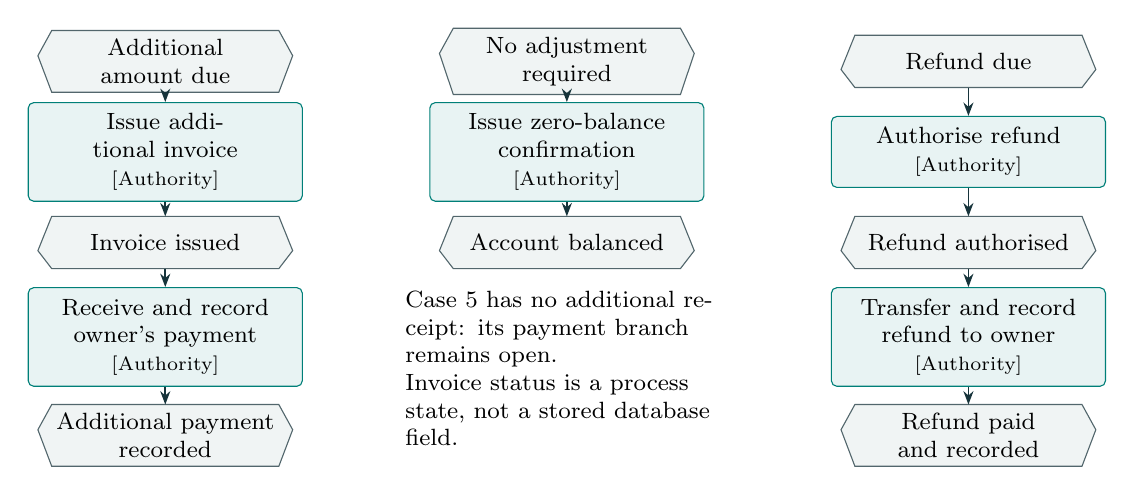
\begin{tikzpicture}[function/.append style={text width=3.2cm},event/.append style={text width=2.8cm}]
\node[event] (a) at (0,0) {Additional\\amount due};
\node[function] (b) at (0,-1.15) {Issue additional invoice\\{\scriptsize [Authority]}};
\node[event] (c) at (0,-2.3) {Invoice issued};
\node[function] (d) at (0,-3.5) {Receive and record\\owner's payment\\{\scriptsize [Authority]}};
\node[event] (e) at (0,-4.75) {Additional payment\\recorded};
\node[event] (f) at (5.1,0) {No adjustment\\required};
\node[function] (g) at (5.1,-1.15) {Issue zero-balance\\confirmation\\{\scriptsize [Authority]}};
\node[event] (h) at (5.1,-2.3) {Account balanced};
\node[event] (i) at (10.2,0) {Refund due};
\node[function] (j) at (10.2,-1.15) {Authorise refund\\{\scriptsize [Authority]}};
\node[event] (k) at (10.2,-2.3) {Refund authorised};
\node[function] (l) at (10.2,-3.5) {Transfer and record\\refund to owner\\{\scriptsize [Authority]}};
\node[event] (m) at (10.2,-4.75) {Refund paid\\and recorded};
\foreach \s/\t in {a/b,b/c,c/d,d/e,f/g,g/h,i/j,j/k,k/l,l/m} \draw[flow] (\s)--(\t);
\node[align=left,text width=4.1cm,font=\fontsize{8.5}{10}\selectfont] at (5.1,-3.9) {Case 5 has no additional receipt: its payment branch remains open.\\Invoice status is a process state, not a stored database field.};
\end{tikzpicture}
\end{center}
\epclegend
\sources{Continuation from A4, exactly one branch per case. Sample outcomes: cases 1/4 additional paid; 2 refund paid; 3 balanced; 5 additional still unpaid. [D2], [DB].}
\end{frame}

\begin{frame}{A6 | Process 3, part 1: accept only consistent data}
\begin{center}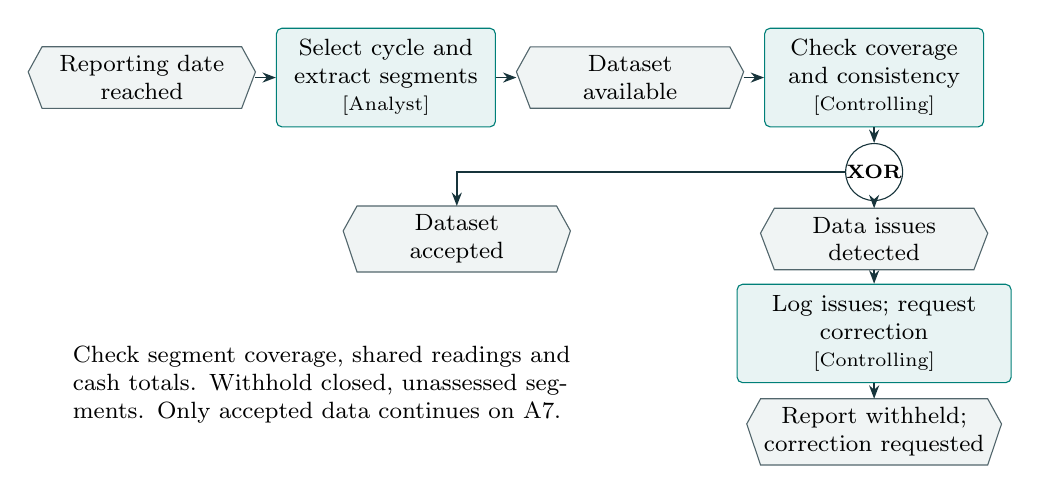
\begin{tikzpicture}[function/.append style={text width=2.5cm},event/.append style={text width=2.45cm}]
\node[event] (a) at (0,0) {Reporting date\\reached};
\node[function] (b) at (3.1,0) {Select cycle and\\extract segments\\{\scriptsize [Analyst]}};
\node[event] (c) at (6.2,0) {Dataset\\available};
\node[function] (d) at (9.3,0) {Check coverage\\and consistency\\{\scriptsize [Controlling]}};
\node[xor] (x) at (9.3,-1.2) {XOR};
\node[event] (ok) at (4,-2.05) {Dataset\\accepted};
\node[event] (bad) at (9.3,-2.05) {Data issues\\detected};
\node[function,text width=3.2cm] (fix) at (9.3,-3.25) {Log issues; request\\correction\\{\scriptsize [Controlling]}};
\node[event,text width=2.8cm] (end) at (9.3,-4.5) {Report withheld;\\correction requested};
\foreach \s/\t in {a/b,b/c,c/d,d/x,x/bad,bad/fix,fix/end} \draw[flow] (\s)--(\t);
\draw[flow] (x.west)-|(ok.north);
\node[align=left,font=\fontsize{8.5}{10}\selectfont,text width=6.8cm,anchor=west] at (-1,-3.9) {Check segment coverage, shared readings and cash totals. Withhold closed, unassessed segments. Only accepted data continues on A7.};
\end{tikzpicture}
\end{center}
\epclegend
\sources{Complete Process 3 spans A6–A7. Extraction and quality review are designed activities; query execution and sample checks were performed locally. [L2]; [L4] PDF pp. 48–49.}
\end{frame}

\begin{frame}{A7 | Process 3, part 2: release information for decisions}
\small
\begin{center}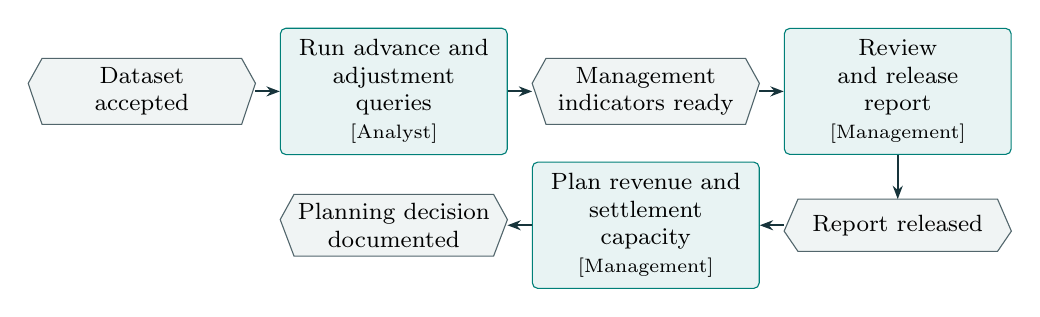
\begin{tikzpicture}[function/.append style={text width=2.6cm},event/.append style={text width=2.45cm}]
\node[event] (a) at (0,0) {Dataset\\accepted};
\node[function] (b) at (3.2,0) {Run advance and\\adjustment queries\\{\scriptsize [Analyst]}};
\node[event] (c) at (6.4,0) {Management\\indicators ready};
\node[function] (d) at (9.6,0) {Review and release\\report\\{\scriptsize [Management]}};
\node[event] (e) at (9.6,-1.7) {Report released};
\node[function] (f) at (6.4,-1.7) {Plan revenue and\\settlement capacity\\{\scriptsize [Management]}};
\node[event] (g) at (3.2,-1.7) {Planning decision\\documented};
\foreach \s/\t in {a/b,b/c,c/d,d/e,e/f,f/g} \draw[flow] (\s)--(\t);
\end{tikzpicture}
\end{center}
\begin{tabularx}{\textwidth}{@{}p{.40\textwidth}X@{}}\toprule
\textbf{Implemented aggregate} & \textbf{Decision enabled}\\\midrule
Estimated advance liability by type/year & Plan advance revenue and understand the declared mileage mix.\\
Gross extra tax/refunds by start year & Plan settlement-processing capacity and scale of adjustments.\\\bottomrule
\end{tabularx}\par
\epclegend
\sources{Continuation from A6. [Q1–Q2] are the two actual analyses. Cash/outstanding reporting is supplementary validation in A21, not the meaning of Q2. [L4] PDF pp. 48–49.}
\end{frame}

\begin{frame}{A8 | Full conceptual ER model: attributes and relationships}
\renewcommand{\erdetail}{1}
\begin{center}% Six conceptual entities. FK attributes appear in the relational dictionary.
% Set \erdetail to 1 before input for the full attribute view.
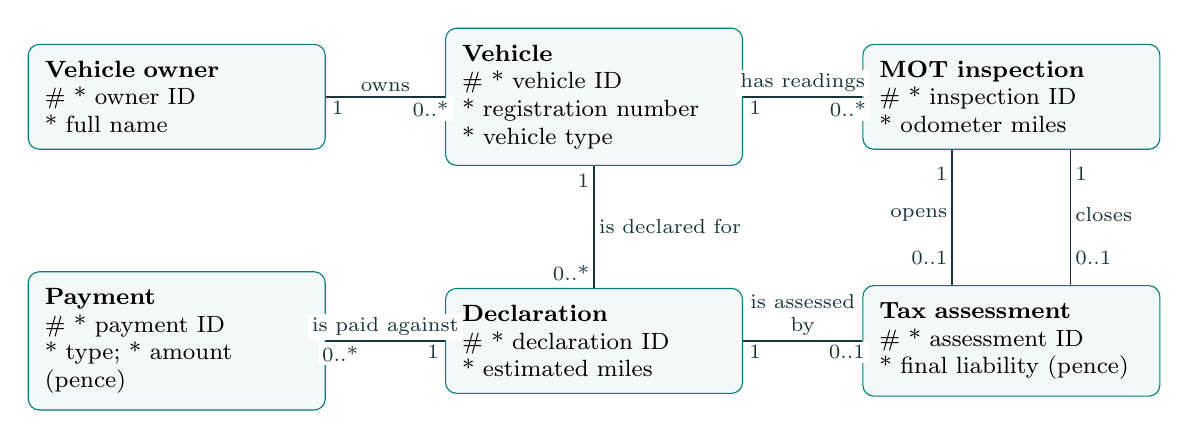
\begin{tikzpicture}
\node[entity] (o) at (0,0) {\textbf{Vehicle owner}\\\# * owner ID\\{}* full name\ifnum\erdetail=1\\{}* postal address\fi};
\node[entity] (v) at (5.3,0) {\textbf{Vehicle}\\\# * vehicle ID\\{}* registration number\\{}* vehicle type};
\node[entity] (i) at (10.6,0) {\textbf{MOT inspection}\\\# * inspection ID\\{}* odometer miles\ifnum\erdetail=1\\{}* inspection date\\{}* centre reference\fi};
\node[entity] (p) at (0,-3.1) {\textbf{Payment}\\\# * payment ID\\{}* type; * amount (pence)\ifnum\erdetail=1\\{}* paid timestamp\fi};
\node[entity] (d) at (5.3,-3.1) {\textbf{Declaration}\\\# * declaration ID\\{}* estimated miles\ifnum\erdetail=1\\{}* period start\\{}* period end (exclusive)\\{}* advance due (pence)\\{}* submitted at\fi};
\node[entity] (a) at (10.6,-3.1) {\textbf{Tax assessment}\\\# * assessment ID\\{}* final liability (pence)\ifnum\erdetail=1\\{}* assessed timestamp\fi};
\draw[relation] (o)--node[relabel,above]{owns} node[relabel,pos=.1,below]{1} node[relabel,pos=.88,below]{0..*}(v);
\draw[relation] (v)--node[relabel,above]{has readings} node[relabel,pos=.1,below]{1} node[relabel,pos=.88,below]{0..*}(i);
\draw[relation] (v)--node[relabel,right]{is declared for} node[relabel,pos=.12,left]{1} node[relabel,pos=.88,left]{0..*}(d);
\draw[relation] (p)--node[relabel,above]{is paid against} node[relabel,pos=.12,below]{0..*} node[relabel,pos=.9,below]{1}(d);
\draw[relation] (d)--node[relabel,above]{is assessed\\by} node[relabel,pos=.1,below]{1} node[relabel,pos=.87,below]{0..1}(a);
\draw[relation] ($(i.south)+(-.75,0)$)--node[relabel,pos=.18,left]{1} node[relabel,pos=.8,left]{0..1} node[relabel,pos=.48,left]{opens} ($(a.north)+(-.75,0)$);
\draw[relation] ($(i.south)+(.75,0)$)--node[relabel,pos=.18,right]{1} node[relabel,pos=.8,right]{0..1} node[relabel,pos=.48,right]{closes} ($(a.north)+(.75,0)$);
\end{tikzpicture}
\end{center}
\erlegend
\sources{All non-FK implementation attributes are represented conceptually; foreign keys implement the named relationships (A10–A14). Endpoint ranges give multiplicity for one entity at the opposite end. [L3] PDF p. 28.}
\end{frame}

\begin{frame}{A9 | Cardinalities, lifecycle and inspection reuse}
\small
\begin{tabularx}{\textwidth}{@{}p{.37\textwidth}X@{}}\toprule
\textbf{Relationship} & \textbf{Meaning and implementation}\\\midrule
Owner 1 — 0..* Vehicle & A vehicle has one owner; an owner can have none or many. Owner changes are outside this model.\\
Vehicle 1 — 0..* Declaration / Inspection & Each declaration/inspection belongs to one vehicle. Multiple periods/readings can exist over time.\\
Declaration 1 — 0..* Payment & Each payment has one declaration; no assessment is needed for an advance.\\
Declaration 1 — 0..1 Assessment & Each assessment has one declaration; a declaration may not yet be assessed. Unique assessment declaration FK.\\
Inspection 1 — 0..1 Assessment, per role & Each assessment requires one opening and one closing reading. Each inspection may be used at most once in each role.\\\bottomrule
\end{tabularx}\par
\medskip
\textbf{Reuse example:} the 1 April 2029 inspection may close 2028/29 \emph{and} open 2029/30. Separate unique opening/closing keys permit reuse across the two roles. The second period is not in the sample.
\sources{[DB] Actual schema constraints. Required distinct readings, same vehicle and chronology are validated assumptions, not guaranteed by these foreign keys. [L3–L4].}
\end{frame}

\begin{frame}{A10 | Relational mapping and dictionary: owners to declarations}
\small
\begin{tabularx}{\textwidth}{@{}p{.27\textwidth}X@{}}\toprule
\textbf{Relation / concept} & \textbf{Columns: type and meaning}\\\midrule
\code{vehicle_owners}\newline Vehicle owner & \code{owner_id} INTEGER PK; \code{full_name}, \code{postal_address} TEXT. Stores the responsible fictional owner.\\\addlinespace
\code{vehicles}\newline Vehicle & \code{vehicle_id} INTEGER PK; \code{owner_id} INTEGER FK → owners; \code{registration_number} TEXT UNIQUE; \code{vehicle_type} TEXT (BEV/PHEV by convention). Rate is not a stored column.\\\addlinespace
\code{declarations}\newline Annual declaration & \code{declaration_id} INTEGER PK; \code{vehicle_id} INTEGER FK → vehicles; \code{period_start}, \code{period_end} TEXT; \code{estimated_miles}, \code{advance_due_pence} INTEGER; \code{submitted_at} TEXT. UNIQUE(vehicle\_id, period\_start).\\\bottomrule
\end{tabularx}\par
\medskip
\textbf{Mapping:} each entity becomes a relation; one-to-many relationships place the foreign key on the many side. No junction table is required.
\par\smallskip
\textbf{Keys and nulls:} each PK is \code{INTEGER PRIMARY KEY}; all other columns are explicitly \code{NOT NULL}. Dates are text values, not a native SQLite date storage class.
\sources{[DB] scripts/setup\_database.py and PRAGMA table\_info/foreign\_key\_list/index\_list. [L3] PDF p. 15; [L4] pp. 15–18.}
\end{frame}

\begin{frame}{A11 | Relational mapping and dictionary: readings to cash}
\small
\begin{tabularx}{\textwidth}{@{}p{.27\textwidth}X@{}}\toprule
\textbf{Relation / concept} & \textbf{Columns: type and meaning}\\\midrule
\code{mot_inspections}\newline MOT inspection & \code{inspection_id} INTEGER PK; \code{vehicle_id} INTEGER FK; \code{inspection_date} TEXT; \code{odometer_miles} INTEGER; \code{mot_centre_ref} TEXT. UNIQUE(vehicle\_id, inspection\_date).\\\addlinespace
\code{tax_assessments}\newline Tax assessment & \code{assessment_id} INTEGER PK; \code{declaration_id} INTEGER FK UNIQUE; \code{opening_inspection_id}, \code{closing_inspection_id} INTEGER FKs, each UNIQUE; \code{assessed_at} TEXT; \code{final_tax_pence} INTEGER.\\\addlinespace
\code{payments}\newline Cash movement & \code{payment_id} INTEGER PK; \code{declaration_id} INTEGER FK; \code{payment_type} TEXT; \code{amount_pence} INTEGER; \code{paid_at} TEXT. Types used: ADVANCE, ADDITIONAL, REFUND.\\\bottomrule
\end{tabularx}\par
\medskip
All non-PK fields are explicitly \code{NOT NULL}. Stored derived amounts provide a simple assessment record, but do not guarantee consistency with mileage/rates. Balances are calculated, not stored columns.
\sources{[DB] Actual schema and metadata; all dates/timestamps are TEXT. No CHECK constraints or triggers validate types, positivity, dates or cross-record business rules. [L4] PDF pp. 15–18.}
\end{frame}

\begin{frame}[fragile]{A12 | Schema evidence: owner and vehicle master data}
\begin{columns}[T,onlytextwidth]
\column{.43\textwidth}
\lstinputlisting[language=SQL,firstline=11,lastline=15]{../scripts/setup_database.py}
\column{.53\textwidth}
\lstinputlisting[language=SQL,firstline=20,lastline=26]{../scripts/setup_database.py}
\end{columns}
\medskip
\textbf{Enforced:} one referenced owner per vehicle (with foreign keys enabled), a unique registration number, mandatory name/address/type.
\par\medskip
\textbf{Not enforced:} type must be BEV/PHEV, authentic registration data, or ownership stability during a period. These are assumptions and verification responsibilities.
\sources{Verbatim CREATE statements from [DB] scripts/setup\_database.py, checked against sqlite\_master. Setup creates tables; scripts/load\_db.py separately inserts the sample.}
\end{frame}

\begin{frame}[fragile]{A13 | Schema evidence: one declaration and reading per key}
\begin{columns}[T,onlytextwidth]
\column{.50\textwidth}
\lstinputlisting[language=SQL,firstline=31,lastline=41]{../scripts/setup_database.py}
\column{.46\textwidth}
\lstinputlisting[language=SQL,firstline=46,lastline=54]{../scripts/setup_database.py}
\end{columns}
\medskip
\textbf{Uniqueness is precise:} one declaration per vehicle and \emph{start date}, not an automatic rule against overlapping periods; one inspection per vehicle and inspection date.
\par\smallskip
Dates, mileage order and the validity of the period still need business checks.
\sources{Verbatim CREATE statements from [DB], checked against metadata. The sample uses one fixed 2028/29 period. Foreign keys are enabled in setup and loading connections.}
\end{frame}

\begin{frame}[fragile]{A14 | Schema evidence: assessment is optional; payments are many}
\begin{columns}[T,onlytextwidth]
\column{.57\textwidth}
\lstinputlisting[language=SQL,basicstyle=\linespread{1}\ttfamily\fontsize{7.3}{9}\selectfont,firstline=59,lastline=69]{../scripts/setup_database.py}
\column{.39\textwidth}
\lstinputlisting[language=SQL,basicstyle=\linespread{1}\ttfamily\fontsize{7.3}{9}\selectfont,firstline=74,lastline=81]{../scripts/setup_database.py}
\end{columns}
\medskip
\textbf{Why keep both entities?} The final liability is a tax decision; payments are completed cash movements. A declaration can have an advance before an assessment exists.
\par\smallskip
Each inspection FK is independently unique. The schema does not require the two inspection IDs to differ or belong to the declaration's vehicle.
\sources{Verbatim CREATE statements from [DB]. Integrity check = ok; foreign-key check = no violations. These results do not certify the omitted business rules.}
\end{frame}

\begin{frame}{A15 | Five business cases: declarations and verified miles}
\begin{center}
\begin{tabular}{@{}clrrrr@{}}\toprule
Case & Type & Estimated miles & Opening miles & Closing miles & Actual miles\\\midrule
1 & BEV & 10,000 & 20,000 & 32,000 & 12,000\\
2 & BEV & 10,000 & 40,000 & 48,000 & 8,000\\
3 & BEV & 10,000 & 15,000 & 25,000 & 10,000\\
4 & PHEV & 8,000 & 30,000 & 40,000 & 10,000\\
5 & PHEV & 10,000 & 10,000 & 22,000 & 12,000\\\bottomrule
\end{tabular}
\end{center}
\textbf{Shared boundaries:} opening 1 April 2028; closing 1 April 2029. Billing dates use the exclusive end convention.
\par\medskip
\textbf{Why these are business cases:} each settlement links an owner, vehicle, annual declaration, two readings, assessment and its payment history. They exercise three outcomes and an unfinished additional-payment path in Process 2.
\sources{[DB] Read-only recomputation from the working database. Case number = declaration ID. 5+5+5+10+5+8 = 38 stored records, not five arbitrary rows.}
\end{frame}

\begin{frame}{A16 | Five business cases: liability, signed cash and open balance}
\small
\begin{center}
\begin{tabular}{@{}crrrrrr@{}}\toprule
Case & Advance due/paid & Final tax & Extra paid & Refund paid & Net cash & Remaining\\\midrule
1 & £300 & £360 & £60 & £0 & £360 & £0\\
2 & £300 & £240 & £0 & £60 & £240 & £0\\
3 & £300 & £300 & £0 & £0 & £300 & £0\\
4 & £120 & £150 & £30 & £0 & £150 & £0\\
5 & £150 & £180 & £0 & £0 & £150 & \alert{£30}\\\midrule
Total & £1,170 & £1,230 & £90 & £60 & £1,200 & £30\\\bottomrule
\end{tabular}
\end{center}
\textbf{Assessments:} gross extra tax £60 + £30 + £30 = £120; gross refund £60; net adjustment £60.
\par\medskip
\textbf{Payments:} all five advances paid on 1 April 2028; two additional payments and one refund on 3 April 2029. Assessments dated 2 April 2029.
\par\smallskip
Refund records contain positive values; the £60 is subtracted to obtain net cash. Case 5 has no extra receipt.
\sources{[DB] sample\_data.sql and actual joined records, independently reconciled. Current sample totals across the billing lifecycle, not cash collected within calendar year 2028.}
\end{frame}

\begin{frame}{A17 | Inserted case 5: one settlement across six relations}
\small
\begin{tabularx}{\textwidth}{@{}p{.26\textwidth}X@{}}\toprule
\textbf{Relation / key} & \textbf{Inserted case evidence}\\\midrule
Owner 5 & Emma Example; 5 Example Road, Birmingham (fictional).\\
Vehicle 5 & owner\_id 5; registration DEMO005; type PHEV.\\
Declaration 5 & vehicle\_id 5; 2028-04-01 to exclusive 2029-04-01; estimate 10,000 miles; advance 15,000 pence.\\
Inspections 9 and 10 & vehicle\_id 5; 10,000 miles on 2028-04-01; 22,000 miles on 2029-04-01; centre DEMO-MOT-05.\\
Assessment 5 & declaration\_id 5; opening ID 9; closing ID 10; final liability 18,000 pence.\\
Payment 5 & declaration\_id 5; ADVANCE; 15,000 pence; received 2028-04-01T10:00:00Z. No ADDITIONAL payment.\\\bottomrule
\end{tabularx}\par
\medskip
This case is assessed but has not completed Process 2's payment branch. The unpaid amount is derived from records; invoice issuance is not persisted in a separate table.
\sources{[DB] database/queries/sample\_data.sql, lines 12, 20, 29, 37, 50–51, 60. Verification replayed the actual schema/inserts in memory and matched every committed row.}
\end{frame}

\begin{frame}[fragile]{A18 | Analysis 1: complete SQL and actual output}
\lstinputlisting{../database/queries/expected_revenue.sql}
\smallskip
\small
\begin{tabular}{@{}lcrrr@{}}\toprule
Start year & Type & Vehicles & Declared miles & Expected revenue GBP\\\midrule
2028 & BEV & 3 & 30,000 & 900.00\\
2028 & PHEV & 2 & 18,000 & 270.00\\\bottomrule
\end{tabular}
\par\smallskip
Column headings abbreviate the SQL aliases. \code{expected_revenue_gbp} means \textbf{estimated advance liability}, grouped by billing-period start year, not final liability or cash receipts.
\sources{[Q1] Exact file, executed read-only. Two joined tables: declarations and vehicles. Rounding here formats sums of already-stored pence as GBP; it is not the mileage tax calculation.}
\end{frame}

\begin{frame}[fragile]{A19 | Analysis 2: complete SQL}
\lstinputlisting[basicstyle=\linespread{1}\ttfamily\fontsize{8.4}{10}\selectfont,emptylines=0]{../database/queries/additional_tax.sql}
\sources{[Q2] Exact file, executed read-only. Two joined tables: declarations and tax\_assessments. The inner join includes assessed declarations only. Results and cash reconciliation: A20.}
\end{frame}

\begin{frame}{A20 | Analysis 2 output and the complete financial reconciliation}
\small
\begin{tabular}{@{}crrrrr@{}}\toprule
Start year & Assessed & Extra cases & Refund cases & Extra tax GBP & Refunds GBP\\\midrule
2028 & 5 & 3 & 1 & 120.00 & 60.00\\\bottomrule
\end{tabular}\par
\medskip
\begin{columns}[T,onlytextwidth]
\column{.50\textwidth}
\begin{tabular}{@{}lr@{}}\toprule
\textbf{Liability measures} & \textbf{GBP}\\\midrule
Estimated advance liability & 1,170\\
Final assessed liability & 1,230\\
Gross additional tax assessed & 120\\
Gross refunds assessed & 60\\\bottomrule
\end{tabular}
\column{.46\textwidth}
\begin{tabular}{@{}lr@{}}\toprule
\textbf{Cash measures} & \textbf{GBP}\\\midrule
Advances received & 1,170\\
Additional payments received & 90\\
Refunds paid (subtract) & 60\\
Net cash received & 1,200\\\bottomrule
\end{tabular}
\end{columns}
\keyline{£1,230 − £1,200 = £30 still receivable}
{\small The cash measures are supplementary verification, not additional columns returned by Analysis 2. All five advances are paid, so due equals received only in this sample.}
\sources{[Q2] Exact result with shortened headings; [DB] reconciled cash totals. Planned workload is 3 extra-tax cases, 1 refund case, and 1 no-adjustment case.}
\end{frame}

\begin{frame}[fragile]{A21 | Supplementary validation: aggregate payments before joining}
\begin{columns}[T,onlytextwidth]
\column{.71\textwidth}
\lstinputlisting[basicstyle=\ttfamily\fontsize{7.5}{9}\selectfont,firstline=3]{assets/outstanding_validation.sql}
\column{.26\textwidth}
\small
\begin{tabular}{@{}cr@{}}\toprule
Case & Remaining\\\midrule
1 & £0\\2 & £0\\3 & £0\\4 & £0\\5 & £30\\\bottomrule
\end{tabular}
\par\medskip
One row per declaration prevents an assessment from being counted again for each payment.
\end{columns}
\sources{Additional validation calculation created for this presentation, executed on the read-only database. Full final/net/remaining outputs are retained in assets/database\_verification.json. Distinct from required Analyses 1 and 2.}
\end{frame}

\begin{frame}{A22 | Sources: assignment and course concepts}
\fontsize{8.4}{10.1}\selectfont
\begin{tabularx}{\textwidth}{@{}p{.07\textwidth}X p{.18\textwidth}@{}}\toprule
ID & \textbf{Source inspected locally} & \textbf{PDF pages used}\\\midrule
C & Stephan Aier \& Jochen Müller, \emph{Cases IKT, HS2026}. Local file: Cases-IKT-HS2026.pdf. & 1–4\\
L1 & HSG, \emph{VL01 Einführung und Modellierung}, HS2026. & 54\\
L2 & HSG, \emph{IKT-2026-VL02} (process modelling). & 21–25\\
E & Software AG, \emph{EPC in ARIS — Cheat Sheet}. Local file: EPC cheat sheet.pdf. & 1 (visually read)\\
L3 & HSG, \emph{VL03 Datenmodellierung 2026}. Local file: 05-VL03-Datenmodellierung-2026.pdf. & 15, 26–31\\
L4 & HSG, \emph{VL04 Datenbanken und BI 2026}. & 15–18, 48–49\\
L5 & HSG, \emph{VL05 Architektur und Integration}, HS2026. & 12, 15–16\\
L6 & HSG, \emph{VL06 IT-Strategie und Enterprise Transformation}, HS2026. & 18\\\bottomrule
\end{tabularx}\par
\medskip
Page references are PDF positions, not necessarily printed slide numbers. Course files were found in the author's Downloads folder and inspected on 9 November 2026. Titles retain their original language; presentation explanations are English.
\sources{Concepts are applied to the case; no external claim about current UK tax law is made. Course materials are referenced, not redistributed with this draft.}
\end{frame}

\begin{frame}{A23 | Sources: project evidence and AI attribution}
\fontsize{8.3}{10.2}\selectfont
\textbf{Project:} Mathis Clément, \emph{ikt-hsg-2026}, working tree at commit \code{a2d2b2a}, inspected 9 November 2026.\\
\url{https://github.com/Mclement197/ikt-hsg-2026}
\begin{description}
\item[S] \code{Scope.md}; context from \code{README.md}, \code{questions.md}.
\item[DB] \code{scripts/setup_database.py}, \code{scripts/load_db.py}; \code{database/electromobility.db}; \code{database/queries/sample_data.sql}.
\item[Q1–Q2] \code{database/queries/expected_revenue.sql}, \code{additional_tax.sql}.
\item[D1–D3] Individual \code{diagrams/business_processes/*.drawio}; [D3] is \code{03_management_reporting.drawio}. ER reference files in \code{diagrams/er_diagram/}.
\item[P] Author-supplied \code{opencode_english_presentation_prompt.md}, 9 November 2026; context of earlier AI assistance and English-first request.
\end{description}
\textbf{AI attribution:} OpenAI GPT-6 Astra, used through OpenCode in this session, assisted with source review, English slides/script, TikZ diagrams, SQL reconciliation and build/layout checks. Earlier model files identify \code{agent="Codex"}; no earlier model version or personal discovery is inferred.
\par\smallskip
The author's final review, personal design claims and separate HSG AI-use declaration remain required. Diagram notation adaptations and presentation-specific corrections are documented in \code{assets/README.md}.
\sources{Editable vector diagrams are newly prepared for this deck using course notation with declared extensions. Existing Metropolis theme retained; original template demonstration content and bibliography are not used.}
\end{frame}

\end{document}
